% !TEX root = ../main.tex
% --+ 11.41 SUMMARY +-----------------------------------------------------------
\begin{frame}{FMT Efficiency}
    \label{11.41::summary}

    \begin{itemize}
        \item
            Initially, our plan was to work with \ef{RG-F run 12933} (10.4 GeV beam, 250 nA), but analysis showed a very poor FMT efficiency.

        \item
            This issue comes from three sources: \ef{alignment}, \ef{reconstruction}, and \ef{geometry}.
    \end{itemize}

    \vspace{-12pt}
    \begin{columns}[onlytextwidth,T]

    \begin{column}{.05\linewidth}\end{column} % Centering column.

    \begin{column}{.49\linewidth}
        \begin{center}
            \begin{figure}[t]
                \centering{
                    \fbox{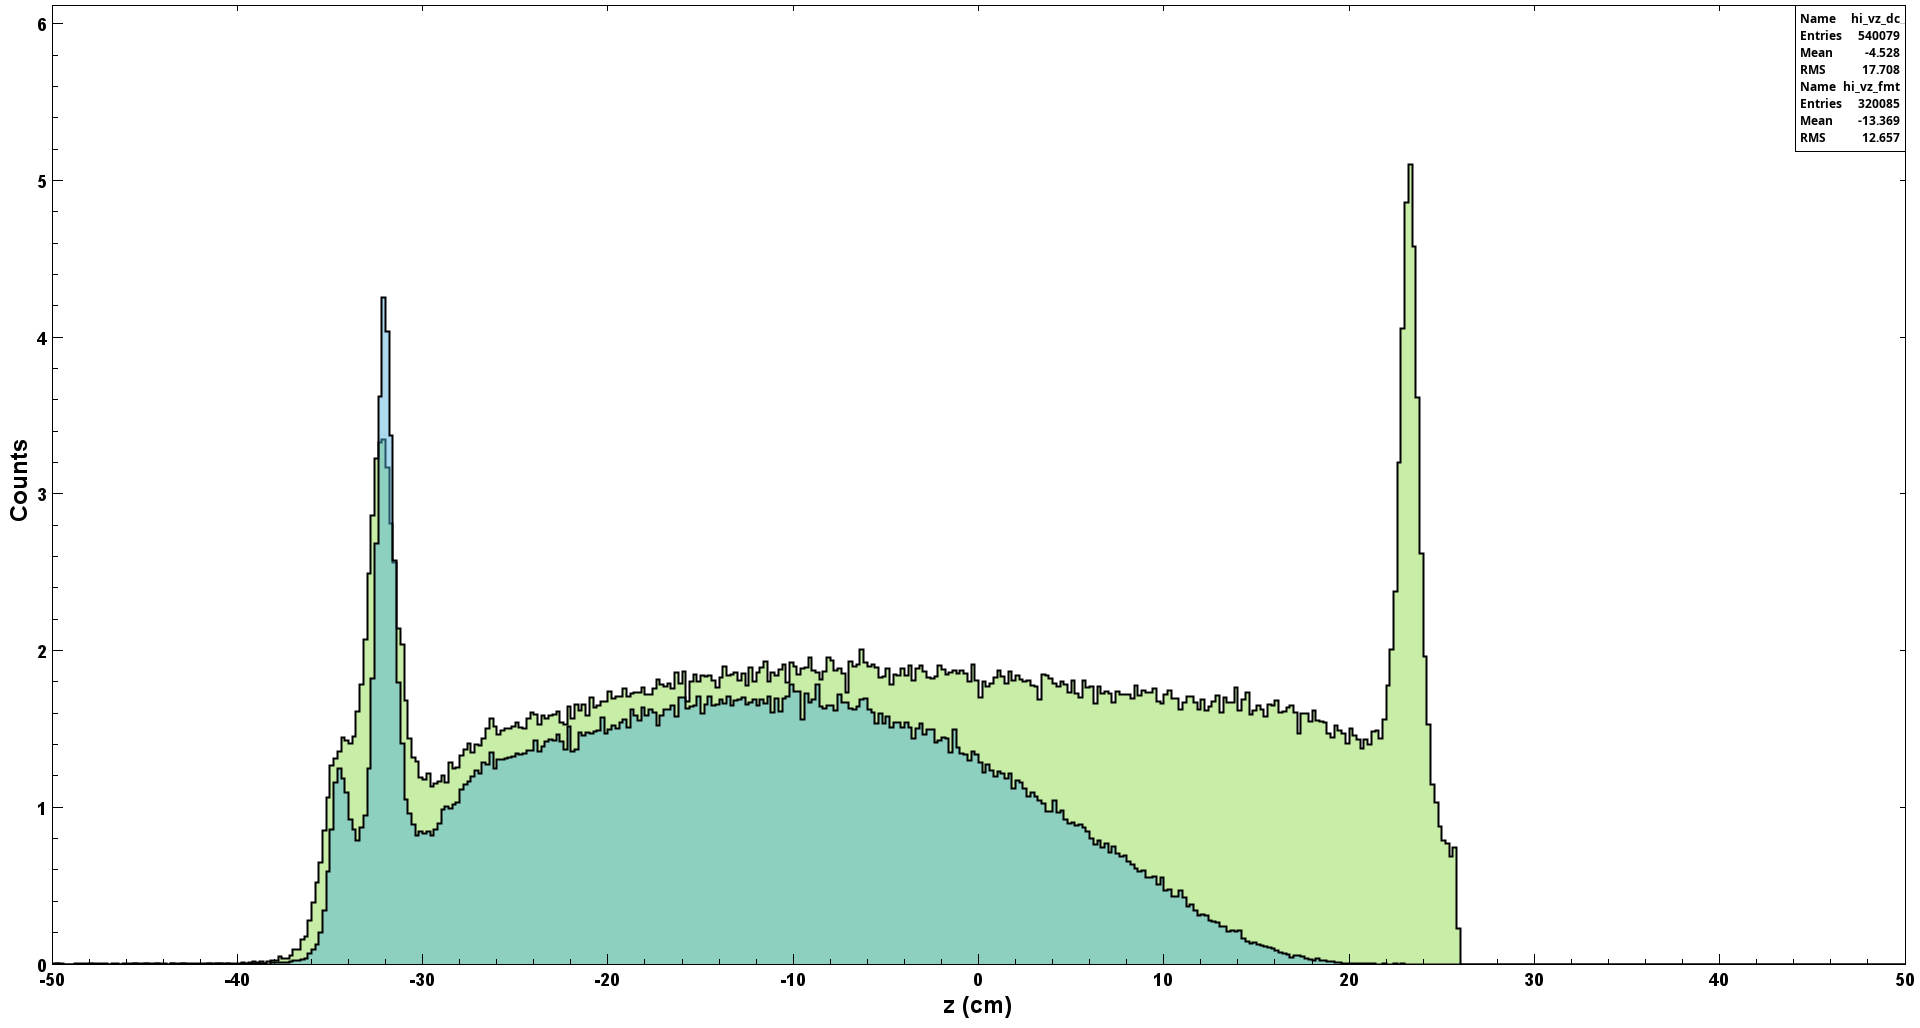
\includegraphics[width=\textwidth]{41vz_011983.png}}
                }
                \scriptsize{\textit{Run \ef{11983}, reconstructed in 2020.}}
            \end{figure}
        \end{center}
    \end{column}

    \begin{column}{.29\linewidth}
        \begin{center}
            \begin{figure}[t]
                \centering{
                    \fbox{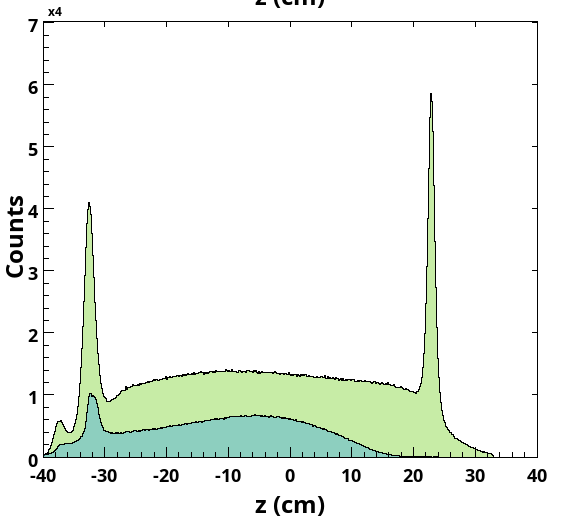
\includegraphics[width=\textwidth]{41vz_012933.png}}
                }
                \scriptsize{\textit{Run \ef{12993}, 2023.}}
            \end{figure}
        \end{center}
    \end{column}

    \begin{column}{.05\linewidth}\end{column} % Centering column.

    \end{columns}
    \begin{center}
        \scriptsize{\textit{
            \ef{$v_z$} for \textbf{\textcolor[HTML]{c7eca6}{DC (green)}} and \textbf{\textcolor[HTML]{8dcfbf}{FMT (cyan)}} tracks.
        }}
    \end{center}
\end{frame}

% --+ 11.42 ALIGNMENT EFFECT +--------------------------------------------------
\begin{frame}{FMT Efficiency: Alignment Effect}
    \label{11.42::alignment_effect}

    \begin{itemize}
        \item
            Alignment problem comes from an issue with the \ef{Summer 2020} alignment table in the Calibration Constants Database\appref{20.07::ccdb}.

        \item
            To work around this, we switch to \ef{Spring 2020} data: \ef{RG-F run 12016}.
    \end{itemize}

    \vspace{-12pt}
    \begin{columns}[onlytextwidth,T]

    \begin{column}{.05\linewidth}\end{column} % Centering column.

    \begin{column}{.35\linewidth}
        \begin{center}
            \begin{figure}[t]
                \centering{
                    \fbox{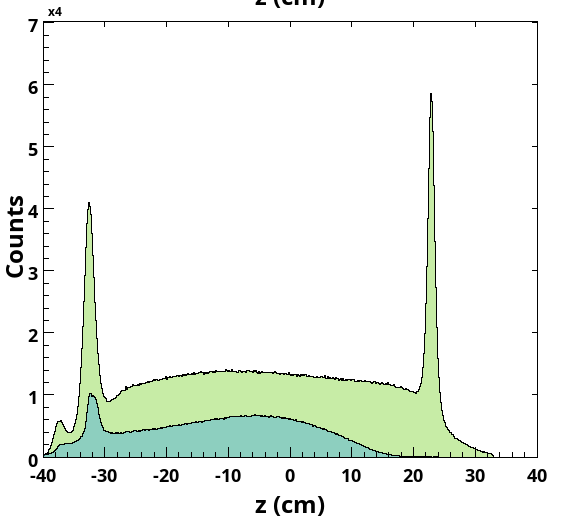
\includegraphics[width=\textwidth]{41vz_012933.png}}
                }
                \scriptsize{\textit{Summer run \ef{12933}.}}
            \end{figure}
        \end{center}
    \end{column}

    \begin{column}{.35\linewidth}
        \begin{center}
            \begin{figure}[t]
                \centering{
                    \fbox{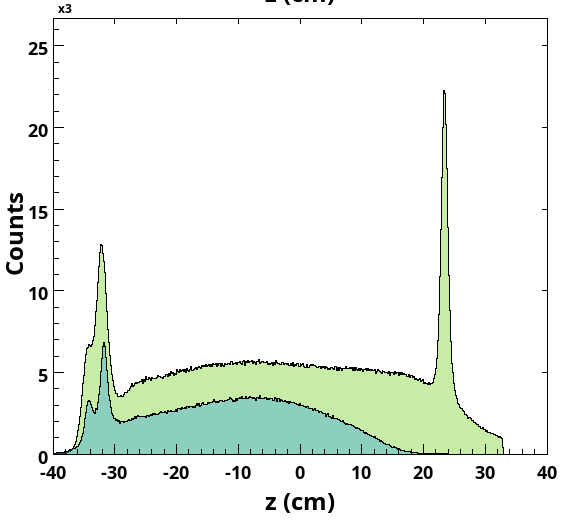
\includegraphics[width=\textwidth]{42vz_012016.png}}
                }
                \scriptsize{\textit{Spring run \ef{12016}.}}
            \end{figure}
        \end{center}
    \end{column}

    \begin{column}{.05\linewidth}\end{column} % Centering column.

    \end{columns}
    \begin{center}
        \scriptsize{\textit{
            \ef{$v_z$} for \textbf{\textcolor[HTML]{c7eca6}{DC (green)}} and \textbf{\textcolor[HTML]{8dcfbf}{FMT (cyan)}} tracks.
        }}
    \end{center}
\end{frame}

% --+ 11.43 GEOMETRY EFFECT 1 +-------------------------------------------------
\begin{frame}{FMT Efficiency: Geometry Effect}
    \label{11.43::geometry_effect_1}

    \begin{itemize}
        \item
            Due to its distance to the target, FMT has a non-trivial efficiency curve along the \ef{$z$ axis} and \ef{$\theta$ angle}.

        \vspace{6pt}
        \item
            If we want to study DIS, we need to understand this effect and disentangle it from the detector's acceptance.
    \end{itemize}

    \vspace{12pt}
    We can define this \ef{efficiency region} by projecting straight lines between the $z$ axis and the detector\appref{20.08::fmt_acceptance_curve}, such that
    \begin{empheq}[box={\eqbox[5pt][5pt]}]{equation*}
        \theta_\text{min}(z) = 57.29^\circ \cdot \text{atan}\left( \frac{R_\text{min}}{z_0 - z} \right),
        \hspace{10pt}
        \theta_\text{max}(z) = 57.29^\circ \cdot \text{atan}\left( \frac{R_\text{max}}{z_0 - z} \right),
    \end{empheq}
    where \ef{$R_\text{min}$} and \ef{$R_\text{max}$} are the radii of FMT, and \ef{$z_0$} is the first layer's $z$ position.

    \vspace{6pt}
    We then apply a cut on DC and FMT tracks based on this region.
\end{frame}

% --+ 11.44 GEOMETRY EFFECT 2 +-------------------------------------------------
\begin{frame}{FMT Efficiency: Geometry Effect}
    \label{11.44::geometry_effect_2}

    Graphically, the correspondance of \efe{$\theta_\text{min}$} and \efe{$\theta_\text{max}$} with FMT's acceptance is evident.

    \begin{center}
        \begin{figure}[t]
            \centering{
                \fbox{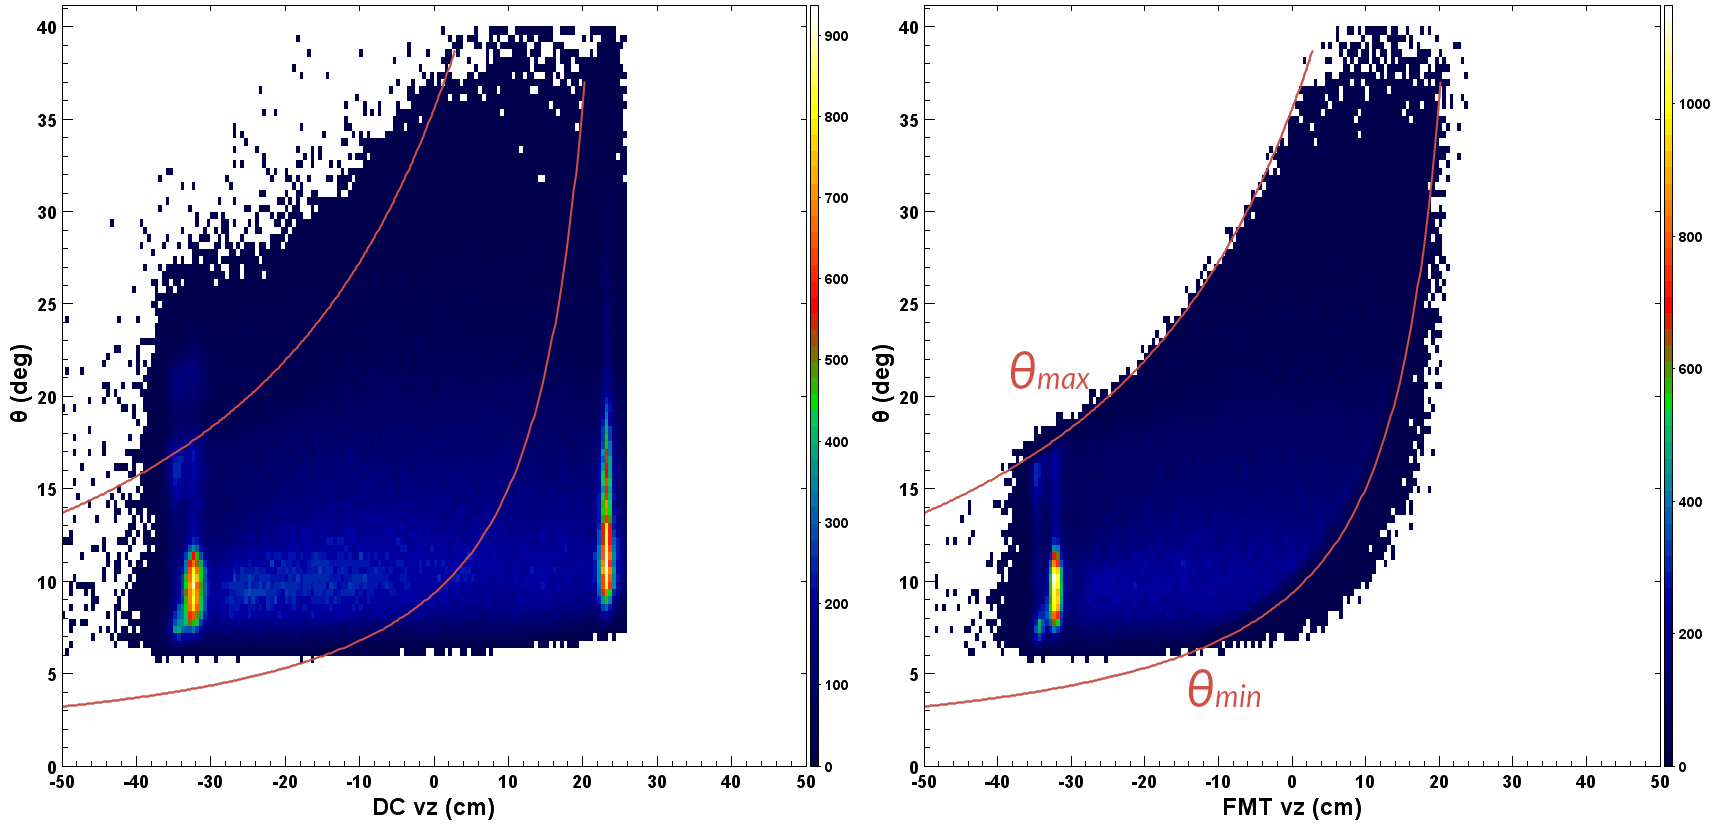
\includegraphics[width=0.9\textwidth]{44vz_theta.png}}
            }
        \end{figure}
        \scriptsize{\textit{
            \efe{$v_z$} vs. \efe{$\theta$} for DC and FMT.
            The \efe{$\theta_\text{min}$} and \efe{$\theta_\text{max}$} curves are highlighted in red.
        }}
    \end{center}
\end{frame}

% --+ 11.45 RECONSTRUCTION EFFECT +---------------------------------------------
\begin{frame}{FMT Efficiency: Reconstruction Effect}
    \label{11.45::reconstruction_effect}

    \begin{itemize}
        \item
            After both corrections, efficiency remains lower than previous measurements.

        \item
            we determined that this effect is not correlated with run number, beam energy, or beam luminosity.
            Thus, \ef{it is attributed to reconstruction}.

        \item
            We define FMT efficiency as the \ef{\% of DC tracks that get accepted by FMT}\appref{20.03::fmt_efficiency_error_estimation}, to see:
    \end{itemize}

    \begin{center}
        \begin{tabularx}{0.76\textwidth}{Xlcrcrr}
            \toprule
            & & & \ef{Run 12933}  & & \multicolumn{2}{c}{\ef{Run 12016}} \\
            & & & \textbf{no cut} & & \textbf{no cut} & \textbf{w/ cut}  \\
            \midrule \midrule
            \ef{$e^-$}      & \textbf{2 layers} & & $25.1 \pm 1.5$ & & $32.7 \pm 2.5$ & $53.7 \pm 0.8$ \\
                            & \textbf{3 layers} & & $ 5.6 \pm 2.7$ & & $ 9.9 \pm 6.3$ & $16.4 \pm 3.6$ \\
            \midrule
            \ef{$e^-\pi^+$} & \textbf{2 layers} & & $ 6.5 \pm 0.2$ & & $11.1 \pm 0.2$ & $28.0 \pm 1.3$ \\
                            & \textbf{3 layers} & & $ 0.3 \pm 0.1$ & & $ 1.0 \pm 0.1$ & $ 2.7 \pm 1.4$ \\
            \midrule
            \ef{$e^-\pi^-$} & \textbf{2 layers} & & $ 5.6 \pm 0.0$ & & $ 8.9 \pm 0.4$ & $29.5 \pm 1.4$ \\
                            & \textbf{3 layers} & & $ 0.3 \pm 0.0$ & & $ 0.9 \pm 0.3$ & $ 2.9 \pm 1.6$ \\
            \bottomrule
        \end{tabularx}
    \end{center}

    \begin{flushright}
        \tiny{\textit{The full efficiency study is presented in Slides \textcolor{efd_purple}{\ref{20.04::fmt_efficiency_study}} to \textcolor{efd_purple}{\ref{20.04::fmt_efficiency_study_end}}.}}
    \end{flushright}
\end{frame}
